\documentclass[fleqn]{report} 
\usepackage[margin=0.5in]{geometry}
\usepackage{amsmath, amsfonts, graphicx, adjustbox, mcode}
\begin{document}
\title{Numerical Methods 4H Assignment 2 - A two-point boundary value problem}
\author{1107023m}
\date{December 2014}
\maketitle

\section{Question 1}
We use a uniform partition of [0,1] by (N + 1) evenly spaced nodes \\
$0 = x_0 < x_1 < \dots < x_n = 1$ where $x_i = i/N$ then $h = 1/N$ and $x_i = hi.$\\
Let $u_i$ denote $u(x_i)$

\section{Question 2}

At each interior point of [0,1] we have the following formulas:
\begin{equation}
    u^{\prime\prime}(x_i) = \frac{u_{i+1} - 2u_i + u_{i-1}}{h^2} + O(h^2) \\
\end{equation}
\begin{equation}
    u^{\prime}(x_i) = \frac{u_{i+1} - u_{i-1}}{2h} + O(h^2)
\end{equation}
\\
The finite difference approximation for $u(x)$ is now obtained by enforcing the
original equation at each interior node of [0,1] that is:

\begin{equation} 
\begin{split}
&\frac{u_{i+1} - 2u_i + u_{i-1}}{h^2} + exp(u_i)\frac{u_{i+1} - u_{i-1}}{2h} = \mu sin(2 \pi x_i)\\\\
&\iff  2u_{i+1} - 4u_i + 2u_{i-1} + hexp(u_i)(u_{i+1} - u_{i-1}) =  2h^2\mu sin(2 \pi x_i)0\\\\
&\iff u_{i+1}(2 + hexp(u_i)) - 4u_i + u_{i-1}(2 - hexp(u_i)) = 2h^2\mu sin(2 \pi x_i)
\end{split}
\end{equation}
for $i \in [1, N - 1]$

\section{Question 3}

The $O(h^2)$ accurate backwards finite difference formula for $u^{\prime}$ is:
\begin{equation}
\frac{u_{i-2} - 4u_{i-1} + 3u_i}{2h} = u^{\prime}(x_i) + O(h^2)
\end{equation}
\\
Substitute this into the boundary equation $u^{\prime}(1) + u^3(1) = 0$:
\begin{equation}
\begin{split}
&u^{\prime}(1) + u^3(1) = 0\\\\
&\iff u^{\prime}(x_N) + u_N^3 = 0\\\\
&\iff \frac{u_{N-2} - 4u_{N-1} + 3u_N}{2h} + u_N^3 = 0\\
&\implies u_N(2hu_N^2 + 3) - 4u_{N-1} + u_{N-2} = 0
\end{split}
\end{equation}
\\
which is the difference equation for node $x_N$\\\\
The difference equation for node $x_0$ is simply $u_0 = 1$

\section{Question 4}

Let F(u) = 0 be a system of N equations where
\begin{equation}
\begin{split} 
&F_1 = u_{2}(2 + hexp(u_1)) - 4u_1 + (2 - hexp(u_1)) - 2h^2\mu sin(2 \pi x_1) = 0  \\
&\vdots \ \ = \ \ \ \ \ \ \                   \vdots\\
&F_i =  u_{i+1}(2 + hexp(u_i)) - 4u_i + u_{i-1}(2 - hexp(u_i)) - 2h^2\mu sin(2 \pi x_i) = 0  \\
&\vdots \ \ = \ \ \ \ \ \ \                   \vdots\\
    &F_{N-1} =  u_{N}(2 + hexp(u_{N-1})) - 4u_{N-1} + u_{N-2}(2 - hexp(u_{N-1})) - 2h^2\mu sin(2 \pi x_{N-1}) = 0\\
&F_N = u_N(2hu^2_N + 3) - 4u_{N-1} + U_{N-2} = 0\\
    \end{split}
\end{equation}
\\
\\
Then calculating the Jacobian matrix $J$ where entry $J_{ij} = \frac{\partial F_i}{\partial u_j}$:\\

Define the following equations for i $\in$ $[2, n-1]$:\\\\
\indent $L_i = \frac{\partial F_i}{\partial u_{i-1}} = 2 - hexp(u_i)$\\ 
\indent $U_i = \frac{\partial F_i}{\partial u_{i+1}} = 2 + hexp(u_i)$\\
\indent $D_i = \frac{\partial F_i}{\partial u_i} =  (u_{i+1} - u_{i-1})hexp(u_i) -4$\\

\[
 J=
\left[ {\begin{array}{cccccccc}
(u_2 - 1)hexp(u_1) - 4 & 2 +hexp(u_1) & 0 & 0 & \hdots & \hdots & \hdots & 0 \\
L_2 & D_2 & U_2 & 0 & \hdots & \hdots & \hdots & 0 \\ 
0 & L_3 & D_3 & U_3 & 0 & \hdots & \hdots & \hdots \\
\vdots & \vdots & \ddots & \ddots & \ddots & \ddots & \hdots & \hdots\\
\vdots & \vdots & \ddots & L_i & D_i  & U_i & \hdots & \hdots \\
\vdots & \vdots & \ddots & \ddots & \ddots & \ddots & \hdots & \hdots \\
0 & \hdots & \hdots & \hdots & 0 & L_{n-1} & D_{n-1} & U_{n-1} \\
0 & \hdots & \hdots & \hdots & \hdots & 1 & -4 & 6hu^2_n + 3\\
  \end{array} } \right]
\]

\newpage
\section{Question 5}
See file q5.matlab for the same code as below:
\lstinputlisting[language=Matlab, frame=single]{q5.matlab}

\newpage
Plotting each iteration we get the following graph:
\begin{figure}[h!]
\begin{center}
    \centerline{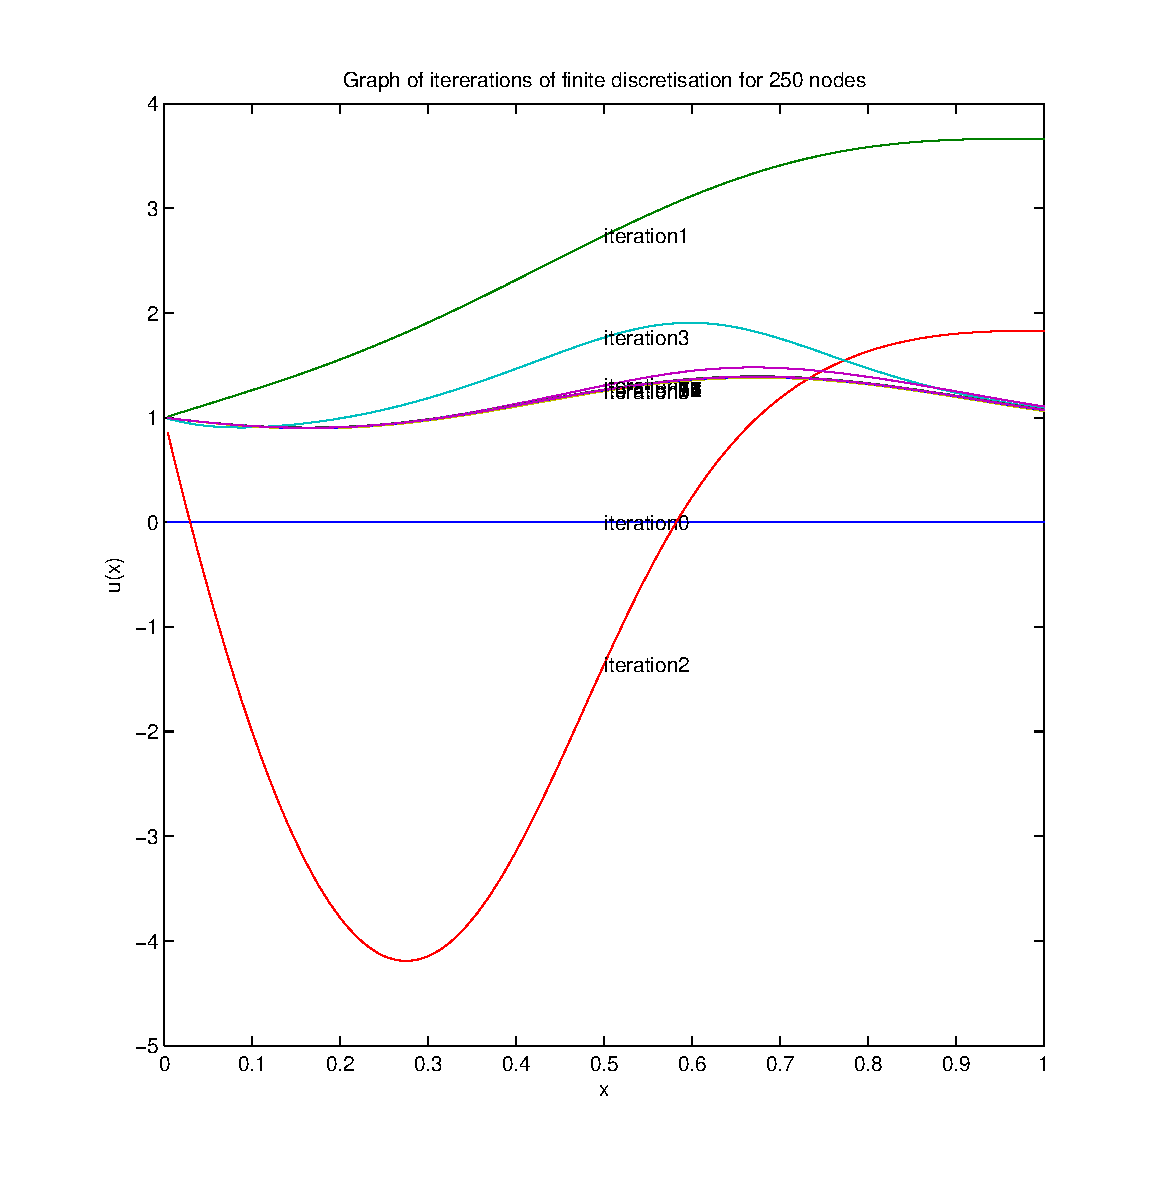
\includegraphics[width=1.1\textwidth]{graphs/q5g1.eps}}
\end{center}
\end{figure}

After around iteration 3 we can clearly see a convergence of values.
\newpage

Zooming in vertically: 
\begin{figure}[h!]
\begin{center}
    \centerline{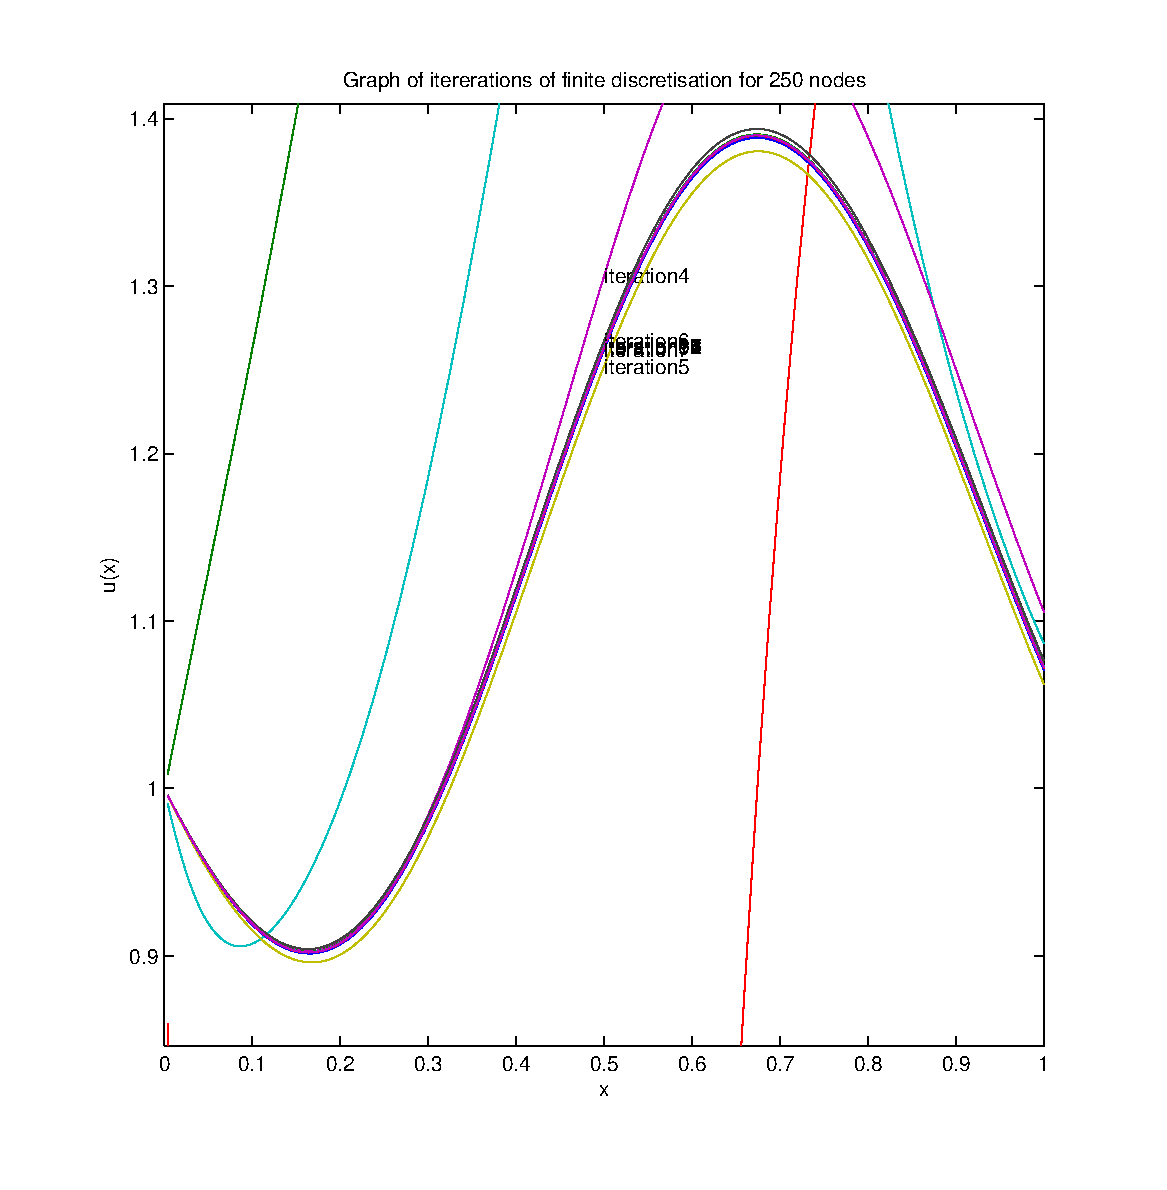
\includegraphics[width=1.1\textwidth]{graphs/q5g2.eps}}
\end{center}
\end{figure}

The convergeance can be seen more clearly as well
as the Newton-Raphson iterations as all values in iteration 4 are larger
than those in iteration 5 and all values in further iterations are inbetween these. 
Zooming in vertically on any further iterations doesn't really give
much information visually without manually scrolling.

\newpage
\section{Question 6}

Modified question 5 matlab code as a function. See file bvp.matlab for
the same code as below:
\lstinputlisting[language=Matlab, frame=single]{bvp.matlab}

See q6.m for matlab code which generates this graph:
\begin{figure}[h!]
\begin{center}
    \centerline{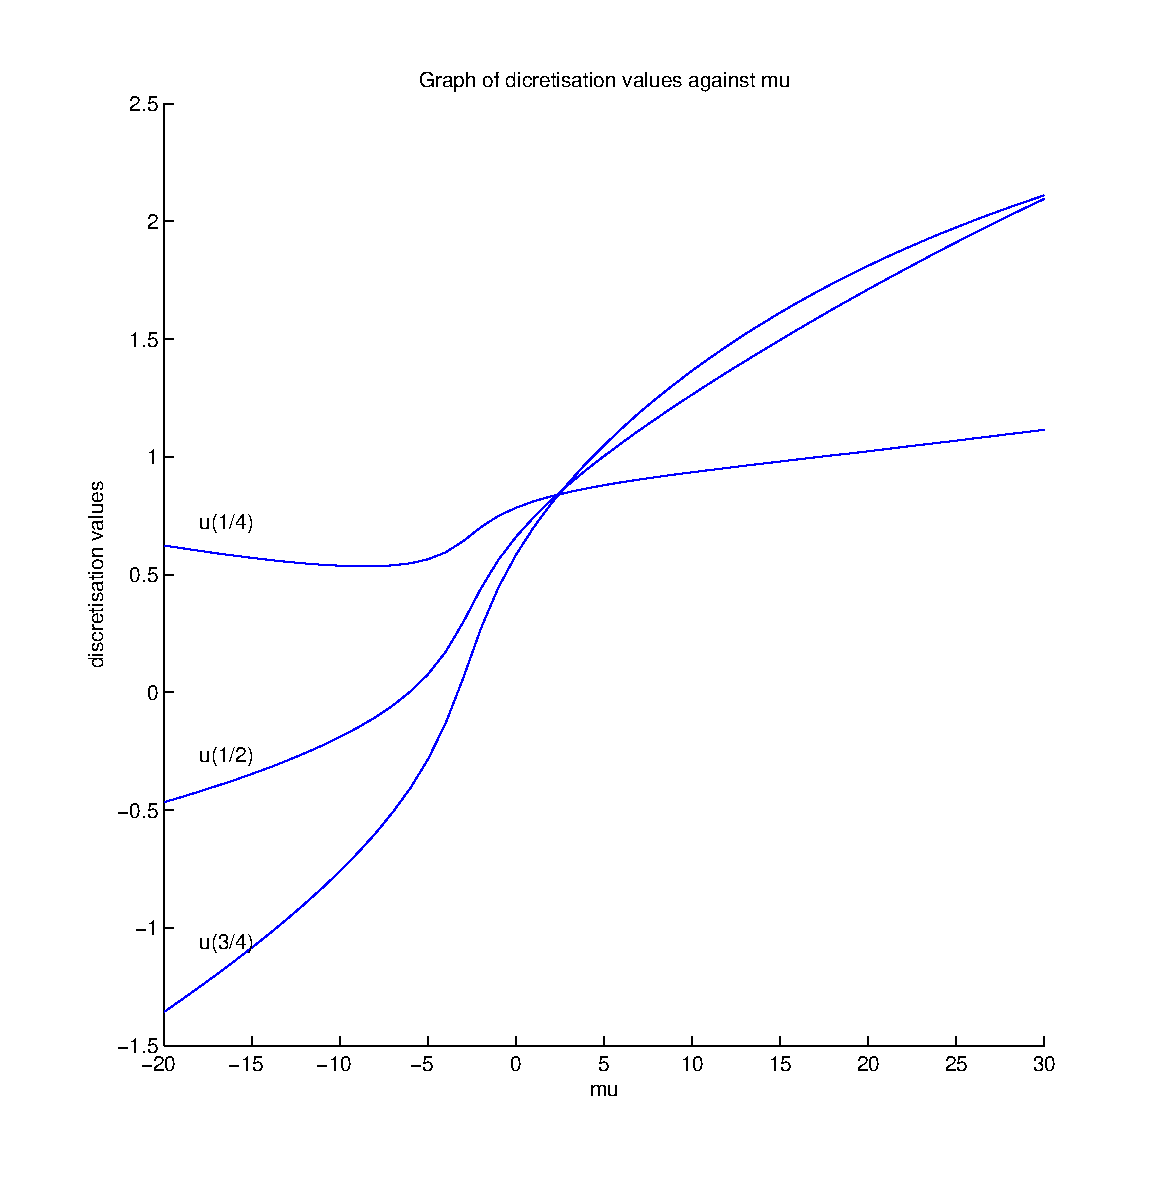
\includegraphics[width=1.0\textwidth]{graphs/q6.eps}}
\end{center}
\end{figure}

\newpage
\section{Question 7}
See q7.matlab for matlab code which generates this graph:
\begin{figure}[h!]
\begin{center}
    \centerline{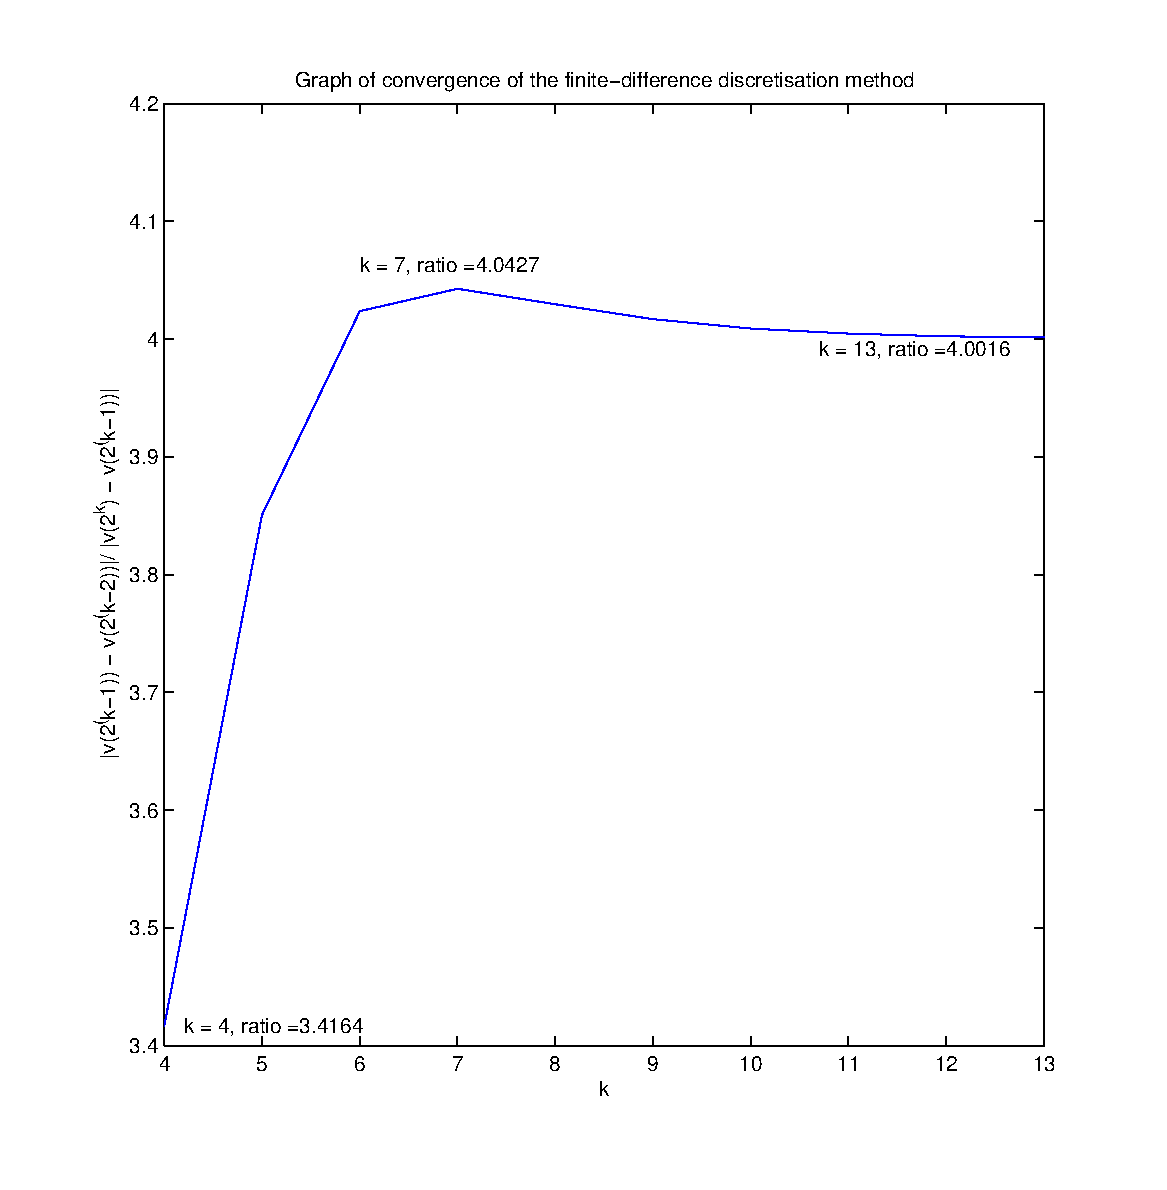
\includegraphics[width=1.0\textwidth]{graphs/q7.eps}}
\end{center}
\end{figure}

\end{document}
